\begin{figure}[h] 
\centering 
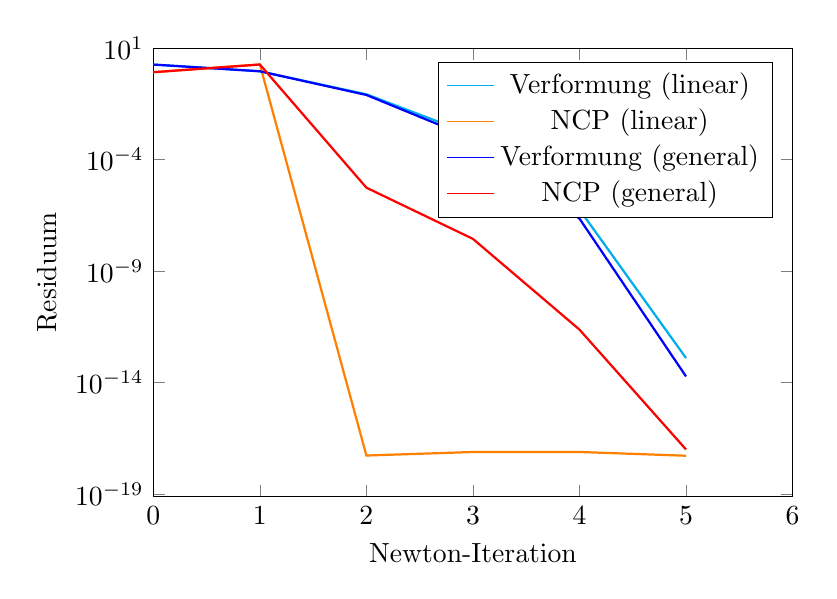
\begin{tikzpicture}[every plot/.append style={thick}] 
\begin{axis}[ 
label style={font=\normalsize}, 
xlabel={Newton-Iteration}, 
ylabel={Residuum}, 
xmin=0, xmax=6, 
ymode=log, 
ymin=0, ymax=10, 
width=0.8\textwidth, 
height=0.6\textwidth, 
legend pos=north east, 
legend style={cells={align=left}}, 
grid style=dashed, 
] 
\addplot[ 
color=cyan, 
] 
coordinates { 
(0, 1.84e+00)(1, 9.19e-01)(2, 8.55e-02)(3, 1.29e-03)(4, 5.78e-07)(5, 1.27e-13)}; 
\addlegendentry{Verformung (linear)} 
\addplot[ 
color=orange, 
] 
coordinates { 
(0, 8.36e-01)(1, 1.86e+00)(2, 5.40e-18)(3, 7.78e-18)(4, 7.79e-18)(5, 5.29e-18)}; 
\addlegendentry{NCP (linear)} 
\addplot[ 
color=blue, 
] 
coordinates { 
(0, 1.84e+00)(1, 9.18e-01)(2, 7.96e-02)(3, 8.72e-04)(4, 2.27e-07)(5, 1.90e-14)}; 
\addlegendentry{Verformung (general)} 
\addplot[ 
color=red, 
] 
coordinates { 
(0, 8.35e-01)(1, 1.85e+00)(2, 5.54e-06)(3, 2.80e-08)(4, 2.39e-12)(5, 1.01e-17)}; 
\addlegendentry{NCP (general)} 
\end{axis} 
\end{tikzpicture} 
\caption{Residuen des Stoffgesetzes 'St.Venant' mit Hinderniss 'Parabel' und 162 Freiheitsgraden für die Verschiebung.} 
\label{fiq:St.Venant_Parabel_level2} 
\end{figure} 
